\documentclass[memoire.tex]{subfiles}

\chapter{Concepts formels}

\section{Introduction}
L'objectif de ce chapitre est dans un premier temps de rappeler des notions de probabilités~\cite{probaBio, decision_tree, apprentissage} qui serviront à la compréhension de ce document. Il s'agit ensuite d'expliquer dans sa généralité les concepts d'arbres décisionnels afin d'introduire des principes d'apprentissage supervisé, de classement et d'optimisation.

\section{Rappels de probabilité}
	\subsection{Expérience aléatoire}
Une expérience est dite aléatoire si les résultats possibles sont connus à l'avance sans vraiment savoir celui obtenu au préalable. On appelle univers, noté \(\Omega\), l'ensemble de toutes les issues possibles d'une expérience et \(\omega\) une réalisation de l'expérience.
\begin{equation}
\Omega = \begin{Bmatrix} \omega_1, \omega_2, \cdots, \omega_n \end{Bmatrix}, n \in \mathbb{N}
\end{equation}
		\subsection{Événements}
Un événement correspond à un ensemble de résultats possibles pour une expérience. Si cet ensemble est constitué d'un seul élément, on parle alors d'événement élémentaire. Si l'ensemble de résultats est égal à l'univers \(\Omega\), alors l'événement est dit certain. En revanche, si aucun résultat n'est présent (ensemble \(\emptyset\)), alors c'est un événement impossible.
		\subsection{Probabilités}
Une probabilité est une fonction qui à un événement $A$, associe un poids.
\begin{equation}
\left \{
\begin{array}{l}
P(\Omega) = 1 \\
P(\emptyset) = 0 \\
0 \leq P(A) \leq 1 \\
P(\bigcup_{i=1}^n A_i) = \sum_{i=1}^n P(A_i)
\end{array}
\right . 
\end{equation}
Plus la probabilité est proche de 1, plus il est possible que l'événement se réalise.
Soit $A$ et $B$ deux événements quelconques, \(P(A)\) est dite conditionnelle si son résultat est influencé par l'événement $B$ :
\begin{equation} 
\left \{
\begin{array}{l}
B \neq \emptyset \\
P(B) \neq 0 \\
A = (A \cap B) \cup (A \cap \overline{B}) \\
\end{array}
\right . 
\end{equation}
On peut alors déduire deux formules : le théorème de Bayes (1.4) permettant de calculer \(P_B(A)\) et le théorème des probabilités totales (1.5) qui permet de connaitre la valeur de \(P(A)\) à partir de deux événements $A$ et $B$. 
\begin{equation}
P_B(A) = \frac{P(A \cap B)}{P(B)}
\end{equation}
\begin{equation}
P(A) = P_B(A)P(B) + P_{\overline{B}}(A)P(\overline{B})
\end{equation}

\section{Arbre de décision}
\subsection{Définition}
Un arbre de décision est une représentation structurelle qui permet d'aboutir à un choix. C'est un graphe acyclique orienté composé :
\begin{itemize}
\item d'un sommet sans parents appelé racine,
\item de sommets appelés nœuds, correspondant à des tests,
\item de sommets terminaux nommés feuilles,
\item des arrêtes, ou branches, désignant chacune les résultats d'un test
\end{itemize}
Pour construire un arbre de décision, une approche \textit{Top-Down} est utilisée, appelée \textit{Top Down Induction of Decision Tree}~\cite{induction_dt} (\textit{TDIDT}). Elle peut se décomposer en plusieurs parties :
\begin{enumerate}
\item Partir du jeu complet de données et construire la racine.
\item Réaliser un test afin de séparer les données.
\item Séparer le nœud actuel en fonction des résultats possibles.
\item Appliquer récursivement jusqu'à atteindre les feuilles.
\end{enumerate}
Lorsque chaque nœud est composé exactement de deux descendants (hors feuilles), on parle alors d'arbre de décision binaire. C'est un cas très largement utilisé des algorithmes de construction d'arbres tels que CART~\cite{ant_colony}, qui sera expliqué ultérieurement.
\subsection{Exemple}
Prenons comme exemple les données météorologiques présentes dans la table 1. Cette table est constituée de différentes colonnes concernant différentes informations ainsi qu'une colonne indiquant si la décision de sortir a été prise ou non. Dans un premier temps, il est possible de déduire les tests à réaliser comme par exemple "La température est-elle élevée ?" ou encore "Quel est le temps ?". De ces questions découlent des réponses possibles, \{oui, non\} pour la première et \{soleil, nuageux, pluie\} pour la deuxième. Une fois l'approche \textit{TDIDT} utilisée, un arbre de décision est alors obtenu (figure 1.1).

\begin{table}[!h]
\footnotesize
\centering
\renewcommand{\arraystretch}{2}
\begin{tabular}{|c|c|c|c|c|c|}
\hline
% thead
Jour &
Temps & 
Température & 
Humidité & 
Vent & 
Sortie\\
\hline
1  & soleil  	& élevée	& haute  	& faible 	& N \\
2  & soleil  	& élevée  	& haute   	& fort 		& N \\
3  & nuageux  	& élevée 	& haute   	& faible 	& Y \\
4  & pluie  	& moyenne   & haute 	& faible 	& Y \\
5  & pluie  	& basse 	& normale 	& faible 	& Y \\
6  & pluie		& basse		& normale   & fort 		& N \\
7  & nuageux	& basse   	& normale 	& fort 		& Y \\
8  & soleil 	& moyenne 	& haute   	& faible 	& N \\
9  & soleil 	& basse  	& normale	& faible 	& Y \\
10 & pluie   	& moyenne 	& normale   & faible 	& Y \\
11 & soleil  	& moyenne   & normale 	& fort	 	& Y \\
12 & nuageux  	& moyenne   & haute 	& fort		& Y \\
13 & nuageux   	& élevée 	& normale 	& faible 	& Y \\
14 & pluie  	& moyenne	& haute   	& fort		& N \\
\hline
\end{tabular}
\caption{Table Météo}
\end{table}

\begin{figure}[!h]
	\centering
	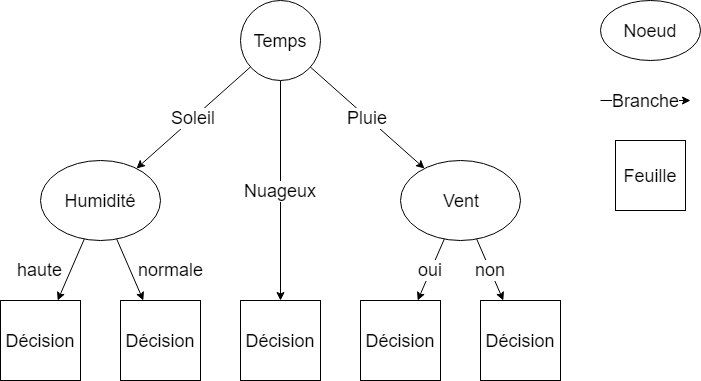
\includegraphics[scale=0.6]{img/decision_tree_meteo.png}
	\caption{Arbre de décision de la table Météo}
\end{figure}

\section{Arbre de décision et classement}
		\subsection{Attributs et classes}
Soit un ensemble d'observations \(S\) de taille \(n\):
\begin{equation}
S = \{s_1, s_2, ..., s_n\}.
\end{equation}
Chaque observation \(s_i\) est composée d'un ensemble de \(m\) attributs :
\begin{equation}
A_s = \{a_1, a_2, ..., a_m\}.
\end{equation}
Soit \(V_j\) l'ensemble de taille \(l\) des valeurs possibles de l'attribut \(a_j\) d'une observation \(s_i\) tel que :
\begin{equation}
V_j = \{ v_1, v_2, ..., v_l \}.
\end{equation}

Un attribut est dit qualitatif si l'ensemble des valeurs possibles est symbolique (non numérique), par exemple si \(V_j\) représente les couleurs d'écriture d'un mot. On obtiendrait alors \( V_j = \{\) bleu, rouge, noir, vert \(\} \):
\begin{itemize}
\item \(a_j\) est nominal si la notion d'ordre n'est pas présente dans l'ensemble des valeurs possibles, par exemple si \(V_j = \{\) un, deux, trois, quatre, cinq, six, sept, huit \(\} \) représente le nom d'un chiffre en toutes lettres.
\item $a_j$ est ordinal si les valeurs possibles contiennent la notion d'ordre. Cela peut être par exemple l'appréciation d'un client : \(V_j = \{\) mauvais, bon, très bon \(\} \)\\

\end{itemize}
\ \\
Une donnée est quantitative si l'ensemble des valeurs possibles est un ensemble numérique fini ou infini :
\begin{itemize}
\item Si un attribut peut prendre une infinité de valeurs dans son ensemble, alors celui-ci est qualifié de continu, par exemple le temps d'exécution d'un processus.
\item Dans le cas contraire, une variable est dite discrète si l'ensemble des valeurs possible est fini. Elle est généralement liée à une énumération, comme par exemple le nombre de traits dans un caractère.
\end{itemize}
\ \\
Qu'elle soit qualitative ou quantitative, une variable est qualifiée de binaire si l'ensemble \(V_j\) des valeurs possibles est de taille \(l=2\), par exemple $V_j = \{0, 1\}$ ou $V_j' = \{ \text{vrai}, \text{faux} \}$\\

La classe d'une observation correspond a une "catégorie" et permet de se rapprocher ou de se différencier des autres observations. Elle correspond à une feuille dans un arbre décisionnel.\\

Reprenons la table 1.1 (Météo), l'attribut \textit{Jour} correspond à l'identifiant d'une observation et donc n'est pas pris en compte. \textit{Temps}, \textit{Température}, \textit{Humidité} et \textit{Vent} sont des attributs qualitatifs. Parmi eux, deux sont binaires : \(V_{Humidite} = \{haute, normale\}\) et \(V_{Vent} = \{fort, faible\} \). Chaque observation possède une classe \textit{Sortie} pouvant prendre Y ou N comme valeur.
		\subsection{Apprentissage supervisé}
Le domaine de l'apprentissage peut se séparer en deux types : le supervisé et le non-supervisé. \\

Dans le cas de l'apprentissage non-supervisé, le but recherché est d'assembler les similitudes entre les observations. Une des méthodes les plus communes est le \textit{clustering}~\cite{data_mining}.\\

Le second type d'apprentissage est dit supervisé. Dans ce cas, le but est d'apprendre du modèle pour arriver à déterminer la classe de l'observation. Ce modèle d'apprentissage est obtenu grâce à des données dont les classes sont connues. Il existe différentes applications de l'apprentissage supervisé, telles que les arbres de décision, les k plus proches voisins et les réseaux de neurones. Nous nous intéresseront uniquement aux arbres de décision et à la méthode des k plus proches voisins. Les jeux de données sont alors séparés en deux : une partie jeu d'entrainement (\textit{training set}) et une partie jeu de test (\textit{test set}). Le but est d'apprendre du jeu d'entrainement afin de classer les observations du jeu de test.\\

Soit $C$ un ensemble de classe de taille $n$ :
\begin{equation}
C = \{c_1, \cdots, c_n\}
\end{equation}
Classer une observation \(s_i\) revient à trouver le \(c_j\) qui lui correspond le mieux par le biais d'une fonction de classement $F$, calculée grâce au jeu de données d'entrainement.
		\subsection{Quantification de l'information}
La composante principale des arbres de décision est la quantification de l'information. "\textit{Dans la théorie de l'information, les notions de quantité d'information et d'incertitude sont équivalentes}"~\cite{decision_tree, information_theory}. Partant de ces concepts, la quantité d'information $h(x)$ d'une probabilité $P(x)$ est une fonction croissante : si $P(x)$ augmente, $h(x)$ augmente. Par ailleurs, les événements certains et impossibles n'apportent aucune information étant donné que le résultat est connu d'avance.\\

Afin de mesurer le gain d'information, il est nécessaire d'introduire le concept d'entropie correspondant à l'impureté d'une observation en théorie de l'information~\cite{theory_communication}. Soit \(S\) un ensemble d'observations de taille \(n\) où \(s_i = \{\text{Y}, \text{N}\}\). L'entropie \(E\) de \(S\), où \(p_Y\) correspond à la probabilité d'avoir \(Y\) et \(p_N\) d'avoir \(N\)~\cite{machine_learning}, est définie par \begin{equation}
E(S) = - p_{Y}log_2p_{Y} - p_{N}log_2p_{N}
\end{equation}
La figure 1.2 représente la fonction d'entropie de S en fonction de $p_Y$. On observe que l'entropie est comprise entre 0 et 1 et vaut 0 lorsque $p_Y$ vaut 0 ou 1. Cela confirme le fait que les événements impossibles et certains n'apportent aucun gain d'information.\\

\begin{figure}[!h]  
\center
\begin{tikzpicture}
\begin{axis}[
    axis lines = left,
    xlabel = $p_t$,
    ylabel = {$E(S)$},
]
\addplot [
    domain=0:1, 
    samples=100, 
    color=black,
]
{-x*log2(x) - (1-x)*log2(1-x) };
\end{axis}
\end{tikzpicture}
\caption{Entropie de $S$ en fonction de $p_t$}
\end{figure}

Nous venons de montrer l'entropie de $S$ pour un attribut binaire. Par extension, si une observation $s_i$ peut prendre $l$ valeurs, alors 
\begin{equation}
E(S) = \sum_{i=1}^{l} - p_ilog_2p_i
\end{equation}

Par exemple, d'après la table 1.1, l'entropie de l'attribut \textit{Sortie} est égale à 
\begin{equation}
\begin{split}
E(Sortie) & = -\frac{9}{14}log_2(\frac{9}{14}) - \frac{5}{14}log_2(\frac{5}{14})\\
		  & = 0.4098 + 0.5305\\
		  & = 0.940
\end{split}
\end{equation}

A partir de cette entropie, il est possible d'obtenir une mesure appelée gain d'information. Celle-ci correspond à la réduction de l'entropie et permet de quantifier l'apport en information lors du choix d'un test. Elle est définie~\cite{machine_learning} par 
\begin{equation}
G(S, A) = E(S) - \sum_{v \in V_A}^{}\frac{|S_v|}{|S|}E(S_v)
\end{equation}

Par exemple, afin de créer l'arbre de décision de la table Météo, il faut déterminer l'attribut qui sera la racine de l'arbre. Pour cela, il faut déterminer quel attribut maximise le gain d'information :\\
\begin{equation}
\begin{split}
& G(S, Temps) = E(S) - \frac{5}{14}E(S_{T, Soleil}) - \frac{4}{14}E(S_{T, Nuageux}) - \frac{5}{14}E(S_{T, Pluie}) = 0.246\\
& G(S, T°) = E(S) - \frac{4}{14}E(S_{Tp, Elev}) - \frac{6}{14}E(S_{Tp, Moy}) - \frac{4}{14}E(S_{Tp, Basse}) = 0.030\\
& G(S, Humidite) = E(S) - \frac{7}{14}E(S_{H, Haute}) - \frac{7}{14}E(S_{H, Normale}) = 0.152\\
& G(S, Vent) = E(S) - \frac{6}{14}E(S_{V, Fort}) - \frac{8}{14}E(S_{V, Faible}) = 0.048\\
\end{split}
\end{equation}
D'après les résultats obtenus :\\ \( G(S, Temps) > G(S, Humidite) > G(S, Vent) > G(S, T°) \). L'attribut \textit{Temps} sera donc choisi comme racine de l'arbre de décision. Ce processus sera ensuite répété pour chaque nouveau nœud crée jusqu'à ce que toutes les feuilles soient atteintes (figure 1.1).

\section{Optimisation d'arbre de décision}
\subsection{Problème d'\textit{overfitting}}
Un des principaux problèmes des arbres de décision est le sur-ajustement (\textit{overfitting}) : la taille d'un arbre augmente linéairement avec la taille du jeu de données d'apprentissage. Ce principe d'\textit{overfitting} peut être défini de la manière suivante : "\textit{soit $H$ un espace d'hypothèses et $h \in H$, $h$ sur-ajuste le jeu d'apprentissage s'il existe une alternative $h' \in H$, tel que h a une marge d'erreur plus petite que $h'$ sur les jeux d'apprentissage, mais une marge d'erreur plus grande sur la totalité du jeux de données.}"~\cite{machine_learning} On peut voir sur la figure 1.3 que plus la précision du jeu d'apprentissage augmente, plus la précision du jeu de test diminue. C'est pourquoi des méthodes d'élagage et d'amélioration d'arbre sont mises en place afin de minimiser ce problème.

\begin{figure}[]
	\centering
	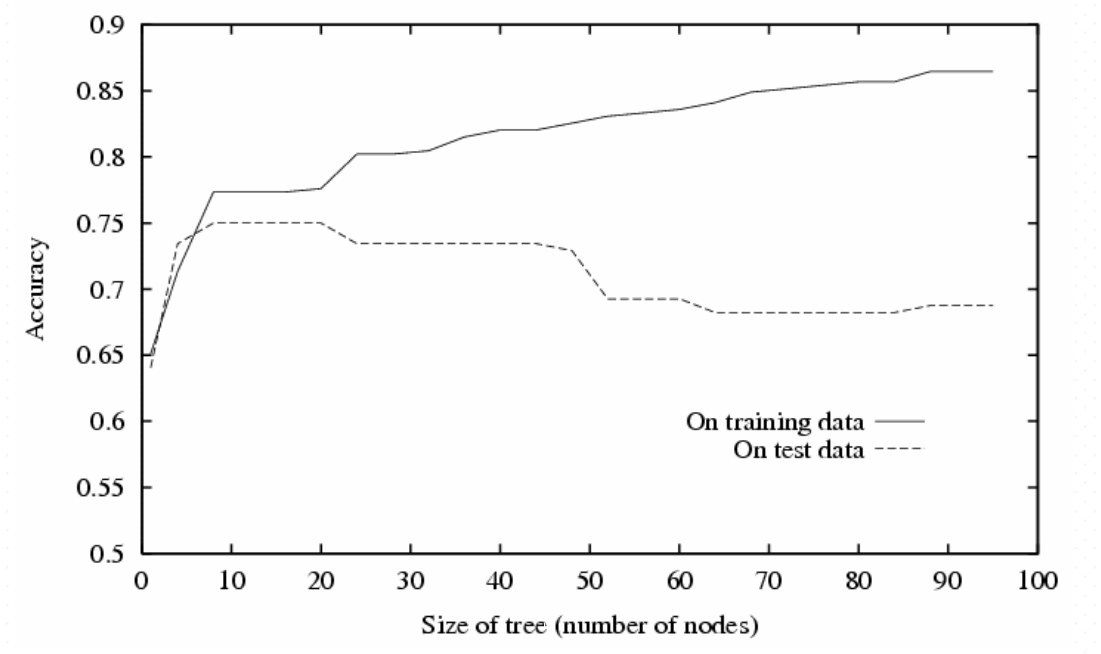
\includegraphics[scale=0.5]{img/overfitting.png}
	\caption{\textit{Overfitting} d'un arbre de décision sur une base de données médicales afin de déterminer si les patients sont atteints de diabète.~\cite{machine_learning}}
\end{figure}

\subsection{Élagage}
\subsubsection{Pré-élagage}
Le pré-élagage consiste à arrêter prématurément la construction de l'arbre même si chaque feuille ne correspond pas à une et seulement une classe. Certains nœuds ne seront alors pas plus développés, selon différents critères d'arrêt choisis au préalable.\\

Une première méthode consiste à définir un nombre d'objets minimum par nœud. Si lors de la création de nouveaux nœuds, l'un d'eux ne dépasse pas le seuil, alors ceux-ci ne sont pas créés et le nœud parent devient une feuille de l'arbre. Une deuxième méthode utilise le test du $\chi^2$ afin de déterminer s'il est statistiquement pertinent de sélectionner un attribut pour construire la suite de l'arbre. Il existe par ailleurs d'autres méthodes qui consistent à définir des seuils pour arrêter la construction~\cite{decision_tree, pruning} :
\begin{itemize}
\item le seuil maximum de feuilles a été atteint,
\item le seuil maximum d'attributs a été franchi,
\item le gain d'information est inférieur à celui fixé. 
\end{itemize}

\subsubsection{Post-élagage}
Contrairement au pré-élagage, le post-élagage se place une fois la construction de l'arbre faite. L'objectif est de supprimer des sous-ensembles de l'arbre afin de les remplacer par des feuilles en minimisant l'impact sur le taux d'erreur, voire réduire le taux d'erreur. Il existe différentes manières d'élaguer un arbre de décision, quatre d'entre elles seront étudiées~\cite{comparative_pruning}.\\

Une première méthode de post-élagage est le \textit{reduced error pruning}~\cite{simplifying_dt}. Elle compare le nombre d'erreur de classement entre le sous-arbre $T_t$ intact et le sous-arbre $T_t'$ lorsque $t$ est transformé en feuille. Si $T_t'$ est plus performant, alors $T_t$ est élagué et $t$ devient une feuille de l'arbre.\\

Le \textit{pessimistic error pruning} est une méthode d'élagage proposée par Quinlan~\cite{simplifying_dt}. Elle remplace le nombre $J$ d'observations mal classées sur une feuille par $J + \frac{1}{2}$. D'après lui, le rapport $\frac{J}{K}$ d'observations mal classées, où K est le nombre d'observations sur une feuille, est une estimation optimiste pas assez fiable, c'est pourquoi il a choisi de la remplacer par une distribution binomiale~\cite{machine_learning, simplifying_dt}.\\

La troisième méthode de post-élagage est le \textit{cost complexity pruning}. Elle consiste à construire une séquence d'arbre $T_0, T_1, \dots, T_L$ en minimisant la valeur de $\alpha$ correspondant à la moyenne du nombre d'observations mal classées par feuille, $T_0$ étant l'arbre initial et $T_L$ l'arbre final. $T_{i+1}$ est obtenu en élaguant tous les nœuds de $T_i$ qui ont la plus petite valeur de $\alpha$~\cite{comparative_pruning}.\\ 

Enfin, le \textit{minimum error pruning} permet de minimiser le taux d'erreur attendu d'un sous-arbre élagué. Si celui-ci est inférieur au taux d'erreur du sous-arbre sans élagage, alors le nœud sera remplacé par une feuille. Ce taux d'erreur est définit par \begin{equation} E_k = \frac{(n - n_j + k - 1)}{n + k} \end{equation} où $n$ correspond au nombre d'observations dans une feuille, $n_j$ observations appartenant à la classe $j$ et $k$ le nombre de valeurs de la classe~\cite{comparative_pruning}.